\providecommand{\main}{../../../..}
\documentclass[\main/dresen_thesis.tex]{subfiles}

\begin{document}
  \section{Grazing-Incidence Small-Angle Neutron Scattering (GISANS)}
    \label{app:methods:gisans}
    The GISANS and polGISANS experiment is basically analogue to GISAXS with the same modifications that have been done when going from SAXS to SANS.
    All presented GISANS experiments in this thesis have been performed on the D33 instrument at ILL \refapp{ch:appendix:lss:d33}.
    \begin{figure}[tb]
      \centering
      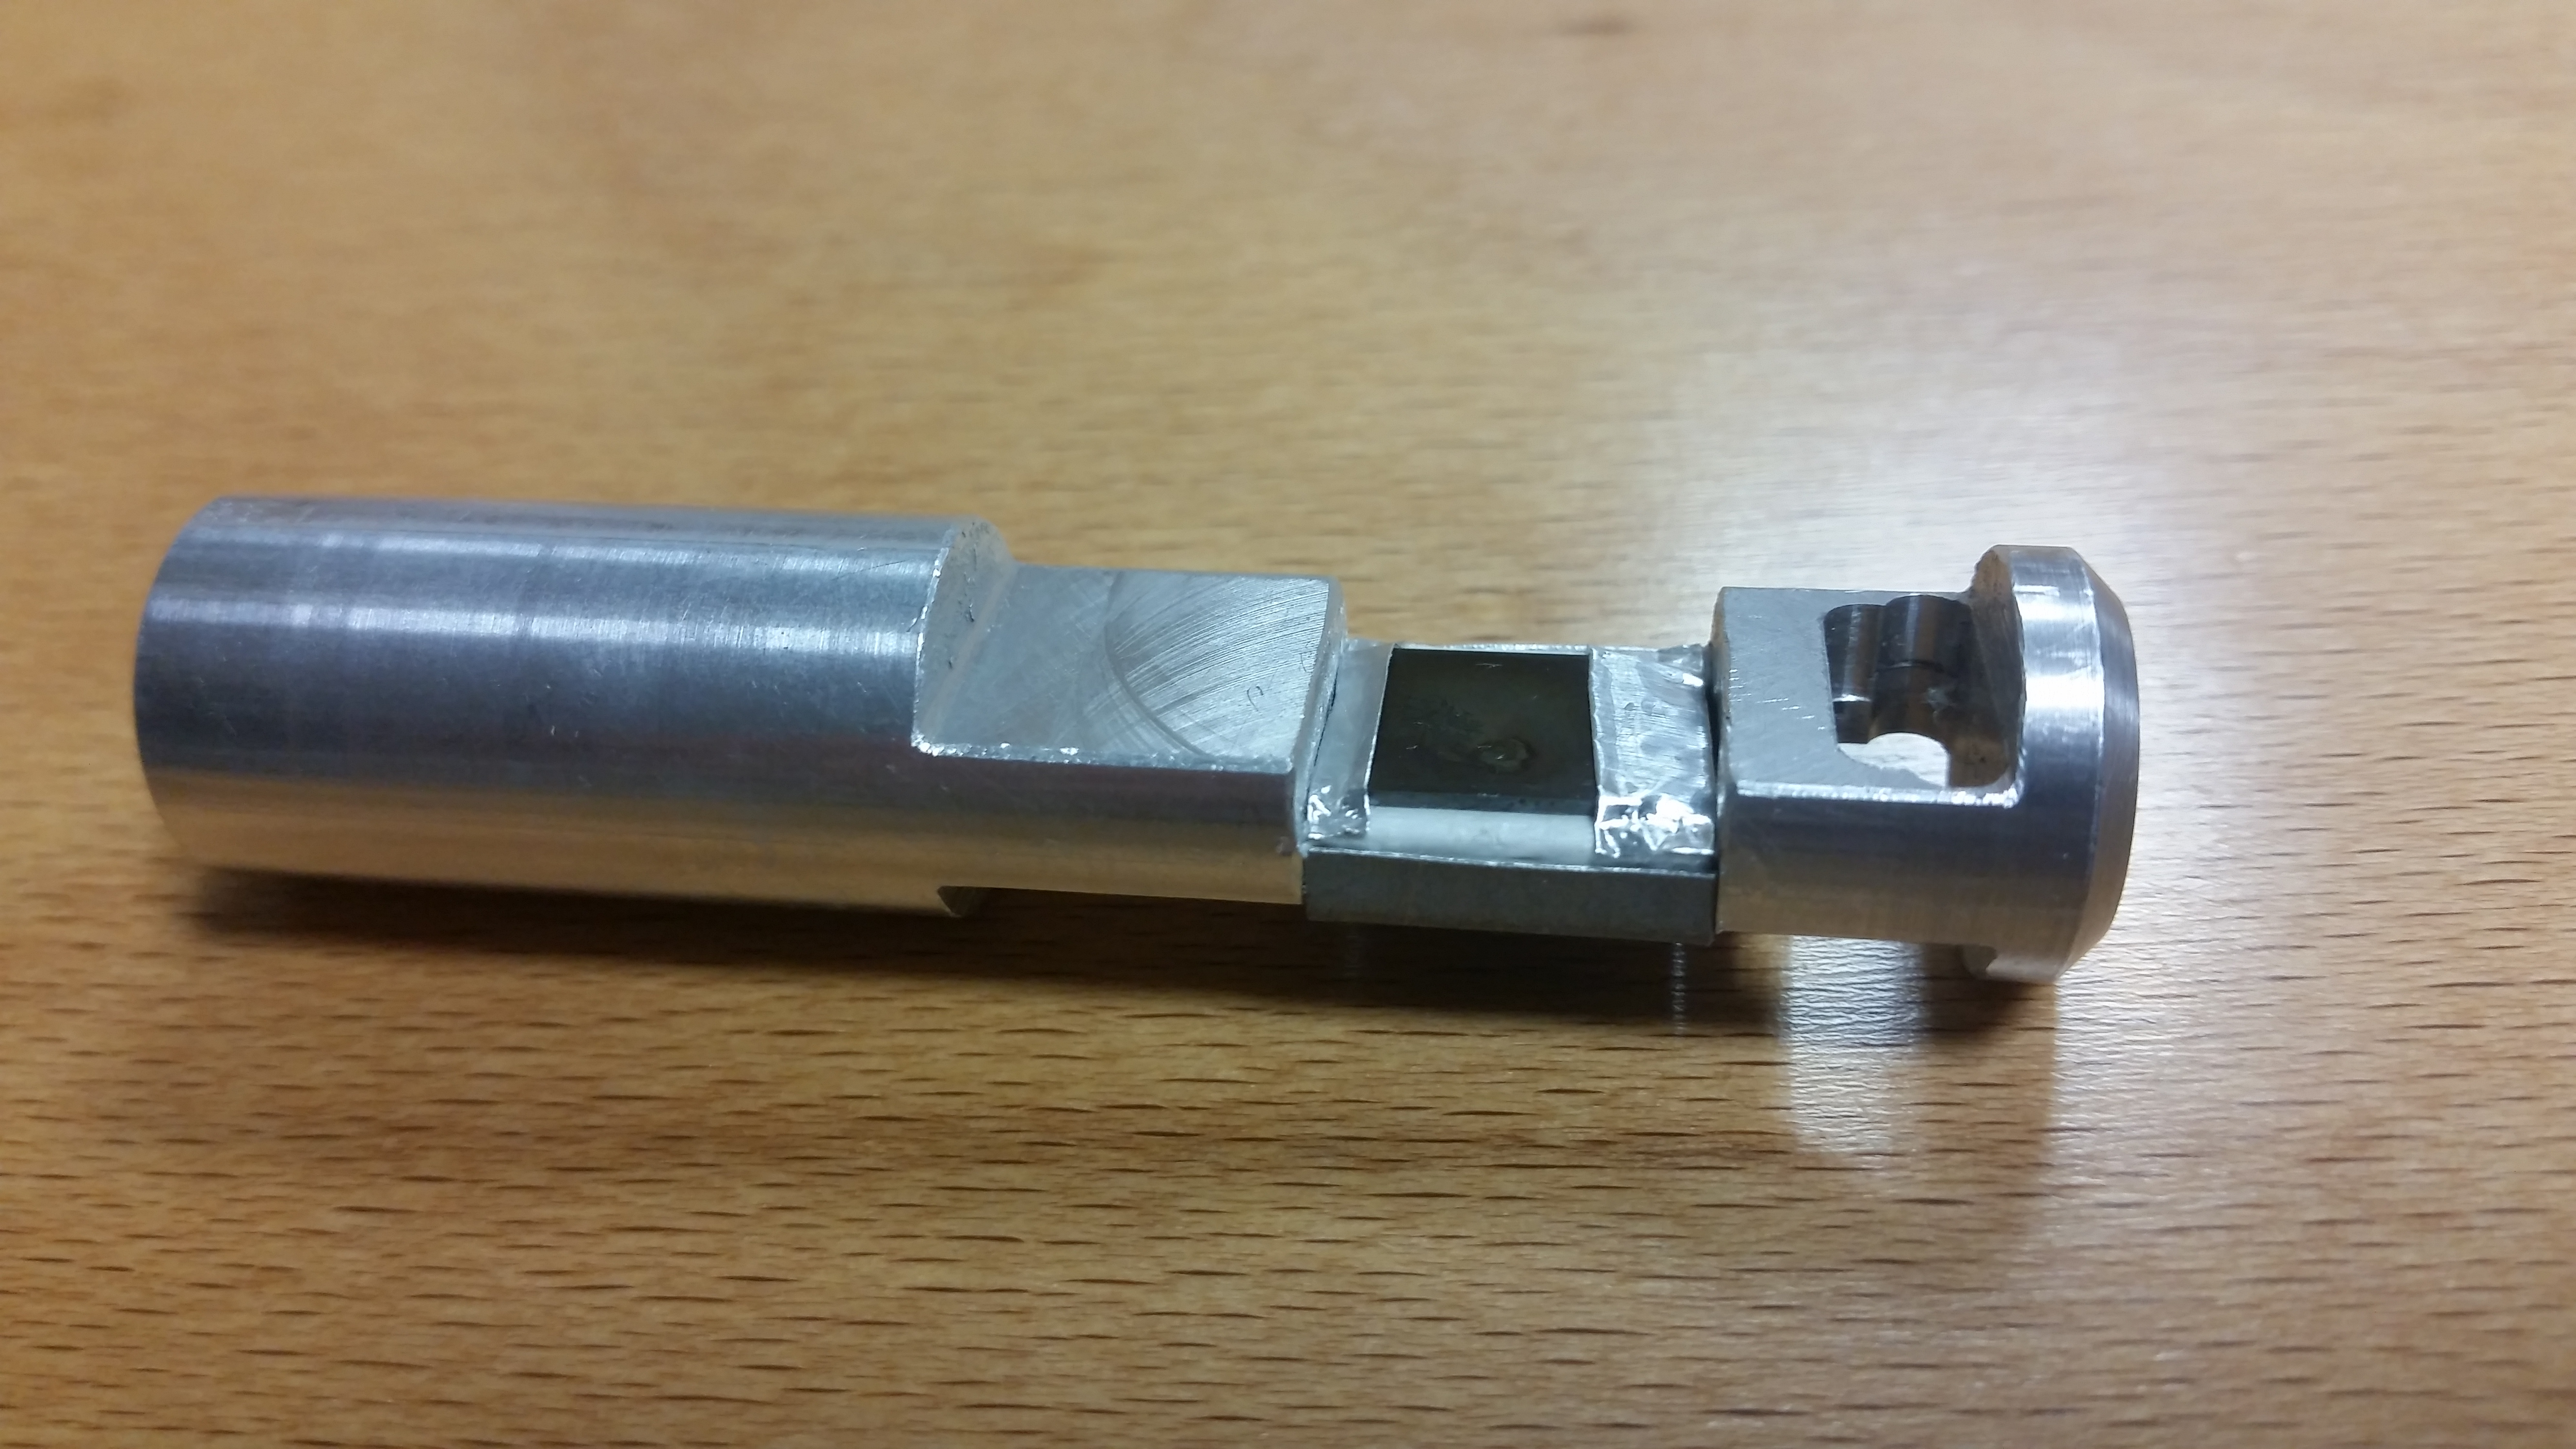
\includegraphics[width=0.7\textwidth]{appendix_methods_gisans_sample}
      \caption{\label{fig:appendix:methods:saxs:samples}In the GISANS experiment, the sample is mounted with sticky tape and aluminium foil on an screwable aluminium holder. To minimize the scattering from the holder and the sticky tape, cadmium stripes are attached on the side below the sample.}
    \end{figure}

    To be able to place the sample in a cryo-magnet, which allows to 
\end{document}